\documentclass[aspectratio=169,11pt]{beamer}
\usetheme{metropolis}
\usepackage{tikz}
\usetikzlibrary{arrows.meta,positioning,decorations.pathmorphing,calc,shapes.geometric,decorations.pathreplacing}
\usepackage{pgfplots}
\pgfplotsset{compat=1.18}
\usepackage{booktabs}
\usepackage{xcolor}

\definecolor{evidence}{HTML}{2196F3}
\definecolor{choice}{HTML}{E91E63}
\definecolor{geometry}{HTML}{4CAF50}
\definecolor{causal}{HTML}{FF9800}
\definecolor{neutral}{HTML}{9E9E9E}
\definecolor{pass}{HTML}{4CAF50}
\definecolor{fail}{HTML}{F44336}
\definecolor{partial}{HTML}{FF9800}
\definecolor{dimhigh}{HTML}{D32F2F}
\definecolor{dimlow}{HTML}{1565C0}

\title{Geometric Structure in Neural Population Codes}
\subtitle{A tool-comparison framework for causal neural geometry\\{\small Exploratory results on Steinmetz 2019}}
\author{Elliot Tower}
\date{2026}
\institute{}

\begin{document}

\maketitle

%% ============================================================
%% SLIDE 2: MOTIVATION — framed around metric disagreement
%% ============================================================

\begin{frame}{Two tools, opposite answers}
\begin{columns}[T]
\begin{column}{0.55\textwidth}
Two standard methods for measuring neural similarity---CKA (linear kernel alignment) and Procrustes (manifold shape distance)---are routinely used interchangeably. We show they systematically disagree, and that effective dimensionality explains why.

\vspace{0.8em}
\textbf{This matters:} which metric you use determines what you conclude about which brain regions ``match.''

\vspace{0.8em}
We then test whether the geometry is causally meaningful using interchange interventions, validated against criteria from philosophy of science.
\end{column}
\begin{column}{0.42\textwidth}
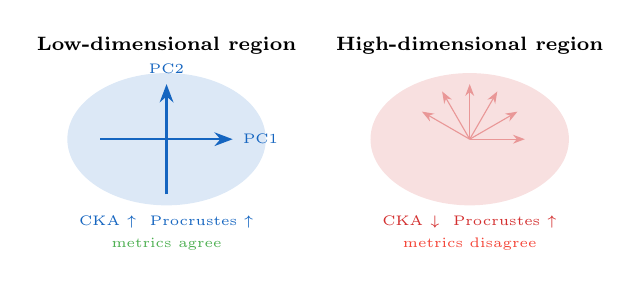
\begin{tikzpicture}[scale=0.7]
  % Panel 1: low-D region (agree)
  \node[font=\scriptsize\bfseries] at (0,3.5) {Low-dimensional region};
  \fill[dimlow!15] (0,1.8) ellipse (1.8 and 1.2);
  \draw[dimlow,thick,-{Stealth}] (-1.2,1.8) -- (1.2,1.8) node[right,font=\tiny] {PC1};
  \draw[dimlow,thick,-{Stealth}] (0,0.8) -- (0,2.8) node[above,font=\tiny] {PC2};
  \node[font=\tiny,dimlow] at (0,0.3) {CKA $\uparrow$ \ Procrustes $\uparrow$};
  \node[font=\tiny,pass] at (0,-0.1) {metrics agree};

  % Panel 2: high-D region (disagree)
  \node[font=\scriptsize\bfseries] at (5.5,3.5) {High-dimensional region};
  \fill[dimhigh!15] (5.5,1.8) ellipse (1.8 and 1.2);
  \foreach \a in {0,30,...,150} {
    \draw[dimhigh!50,thin,-{Stealth[length=1.5mm]}]
      (5.5,1.8) -- +(\a:1.0);
  }
  \node[font=\tiny,dimhigh] at (5.5,0.3) {CKA $\downarrow$ \ Procrustes $\uparrow$};
  \node[font=\tiny,fail] at (5.5,-0.1) {metrics disagree};
\end{tikzpicture}
\end{column}
\end{columns}
\end{frame}

%% ============================================================
%% SLIDE 3: DATA
%% ============================================================

\begin{frame}{The data: Steinmetz et al.\ 2019}
\begin{columns}[T]
\begin{column}{0.5\textwidth}
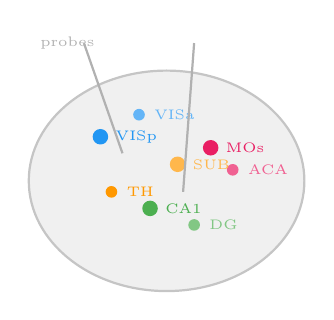
\begin{tikzpicture}[scale=0.7]
  \fill[neutral!15] (0,0) ellipse (2.5 and 2);
  \draw[neutral!60,thick] (0,0) ellipse (2.5 and 2);
  \fill[evidence] (-1.2,0.8) circle (4pt) node[right,font=\tiny,xshift=2pt] {VISp};
  \fill[evidence!70] (-0.5,1.2) circle (3pt) node[right,font=\tiny,xshift=2pt] {VISa};
  \fill[choice] (0.8,0.6) circle (4pt) node[right,font=\tiny,xshift=2pt] {MOs};
  \fill[choice!70] (1.2,0.2) circle (3pt) node[right,font=\tiny,xshift=2pt] {ACA};
  \fill[geometry] (-0.3,-0.5) circle (4pt) node[right,font=\tiny,xshift=2pt] {CA1};
  \fill[geometry!70] (0.5,-0.8) circle (3pt) node[right,font=\tiny,xshift=2pt] {DG};
  \fill[causal] (-1.0,-0.2) circle (3pt) node[right,font=\tiny,xshift=2pt] {TH};
  \fill[causal!70] (0.2,0.3) circle (4pt) node[right,font=\tiny,xshift=2pt] {SUB};
  \draw[neutral!80,thick] (-1.5,2.5) -- (-0.8,0.5);
  \draw[neutral!80,thick] (0.5,2.5) -- (0.3,-0.2);
  \node[font=\tiny,neutral!80] at (-1.8,2.5) {probes};
\end{tikzpicture}
\end{column}
\begin{column}{0.5\textwidth}
\begin{itemize}
  \item 39 sessions, 10 mice
  \item \textbf{73 brain regions} recorded simultaneously
  \item Neuropixels probes (high density)
  \item Visual discrimination task \\
    {\small (which side has higher contrast?)}
  \item 39 sessions $\times$ $\sim$73 regions = \textbf{1,316 pairwise comparisons} for metric analysis
\end{itemize}
\vspace{0.5em}
{\small \textcolor{neutral}{Steinmetz et al., Nature 2019}}
\end{column}
\end{columns}
\end{frame}

%% ============================================================
%% SLIDE 4: CORE FINDING — the three-panel scatter
%% ============================================================

\begin{frame}{CKA and Procrustes systematically disagree}
\begin{columns}[T]
\begin{column}{0.34\textwidth}
\centering
{\scriptsize \textbf{Raw scatter}}
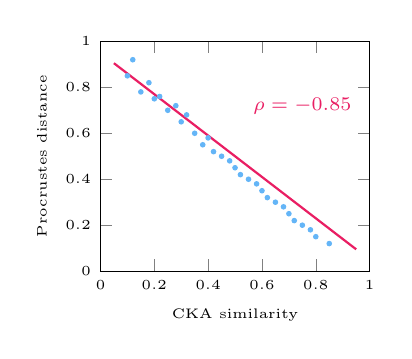
\begin{tikzpicture}
\begin{axis}[
  width=5cm, height=4.5cm,
  xlabel={\tiny CKA similarity},
  ylabel={\tiny Procrustes distance},
  tick label style={font=\tiny},
  xmin=0, xmax=1, ymin=0, ymax=1,
]
  \addplot[only marks, mark=*, mark size=0.8pt, evidence!70]
    coordinates {
      (0.1,0.85)(0.15,0.78)(0.12,0.92)(0.2,0.75)(0.18,0.82)
      (0.25,0.7)(0.22,0.76)(0.3,0.65)(0.28,0.72)(0.35,0.6)
      (0.32,0.68)(0.38,0.55)(0.4,0.58)(0.42,0.52)(0.45,0.5)
      (0.48,0.48)(0.5,0.45)(0.52,0.42)(0.55,0.4)(0.58,0.38)
      (0.6,0.35)(0.62,0.32)(0.65,0.3)(0.68,0.28)(0.7,0.25)
      (0.72,0.22)(0.75,0.2)(0.78,0.18)(0.8,0.15)(0.85,0.12)
    };
  \addplot[choice, thick, domain=0.05:0.95] {0.95 - 0.9*x};
  \node[font=\scriptsize\bfseries,choice] at (axis cs:0.75,0.72) {$\rho = -0.85$};
\end{axis}
\end{tikzpicture}
\end{column}
\begin{column}{0.34\textwidth}
\centering
{\scriptsize \textbf{Colored by eff.\ dimensionality}}
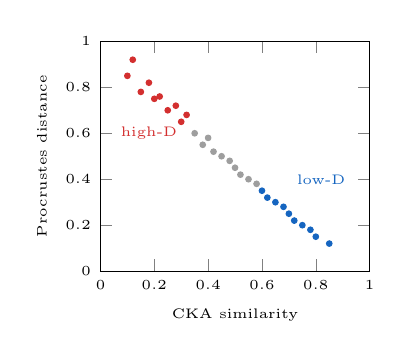
\begin{tikzpicture}
\begin{axis}[
  width=5cm, height=4.5cm,
  xlabel={\tiny CKA similarity},
  ylabel={\tiny Procrustes distance},
  tick label style={font=\tiny},
  xmin=0, xmax=1, ymin=0, ymax=1,
]
  % Low-D points (cool blue) = high CKA, low Procrustes
  \addplot[only marks, mark=*, mark size=1pt, dimlow]
    coordinates {
      (0.7,0.25)(0.72,0.22)(0.75,0.2)(0.78,0.18)(0.8,0.15)(0.85,0.12)
      (0.65,0.3)(0.68,0.28)(0.6,0.35)(0.62,0.32)
    };
  % Mid-D points (neutral)
  \addplot[only marks, mark=*, mark size=1pt, neutral]
    coordinates {
      (0.42,0.52)(0.45,0.5)(0.48,0.48)(0.5,0.45)(0.52,0.42)(0.55,0.4)(0.58,0.38)
      (0.38,0.55)(0.4,0.58)(0.35,0.6)
    };
  % High-D points (warm red) = low CKA, high Procrustes
  \addplot[only marks, mark=*, mark size=1pt, dimhigh]
    coordinates {
      (0.1,0.85)(0.15,0.78)(0.12,0.92)(0.2,0.75)(0.18,0.82)
      (0.25,0.7)(0.22,0.76)(0.3,0.65)(0.28,0.72)(0.32,0.68)
    };
  \node[font=\tiny,dimlow] at (axis cs:0.82,0.4) {low-D};
  \node[font=\tiny,dimhigh] at (axis cs:0.18,0.6) {high-D};
\end{axis}
\end{tikzpicture}
\end{column}
\begin{column}{0.3\textwidth}
\vspace{1em}
{\small The anti-correlation ($\rho = -0.85$) is mediated by effective dimensionality.}

\vspace{0.5em}
{\small Partial $\rho$ controlling for dimensionality: $-0.31$.}

\vspace{0.5em}
{\small High-D regions look ``different'' to CKA and ``similar'' to Procrustes; low-D regions flip.}

\vspace{0.5em}
{\small \textcolor{pass}{\textbf{Replication:}} held from 5 $\to$ 39 sessions}
\end{column}
\end{columns}
\end{frame}

%% ============================================================
%% SLIDE 5: WHY METRICS DISAGREE — mechanistic explanation
%% ============================================================

\begin{frame}{Why CKA and Procrustes disagree}
\begin{columns}[T]
\begin{column}{0.5\textwidth}
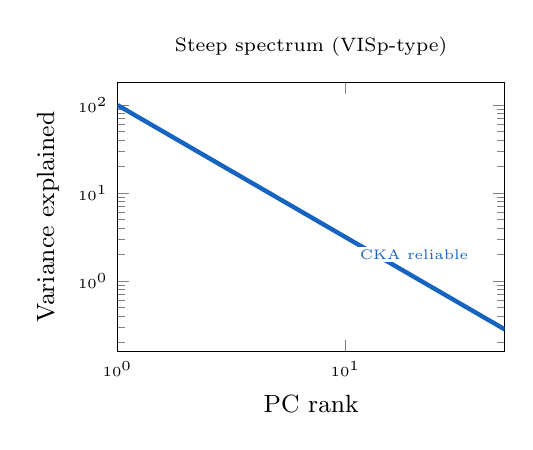
\begin{tikzpicture}
\begin{axis}[
  width=6.5cm, height=5cm,
  xlabel={PC rank},
  ylabel={Variance explained},
  xlabel style={font=\small},
  ylabel style={font=\small},
  tick label style={font=\tiny},
  xmode=log, ymode=log,
  xmin=1, xmax=50,
  title={\scriptsize Steep spectrum (VISp-type)},
  title style={font=\scriptsize},
]
  \addplot[dimlow, ultra thick, domain=1:50, samples=30] {100*x^(-1.5)};
  \node[font=\tiny,dimlow,fill=white,inner sep=1pt] at (axis cs:20,2) {CKA reliable};
\end{axis}
\end{tikzpicture}

\centering{\scriptsize Low-D: dominant eigenvectors stable across animals}
\end{column}
\begin{column}{0.5\textwidth}
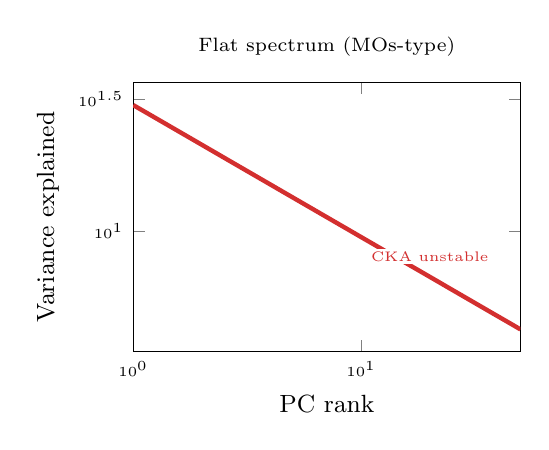
\begin{tikzpicture}
\begin{axis}[
  width=6.5cm, height=5cm,
  xlabel={PC rank},
  ylabel={Variance explained},
  xlabel style={font=\small},
  ylabel style={font=\small},
  tick label style={font=\tiny},
  xmode=log, ymode=log,
  xmin=1, xmax=50,
  title={\scriptsize Flat spectrum (MOs-type)},
  title style={font=\scriptsize},
]
  \addplot[dimhigh, ultra thick, domain=1:50, samples=30] {30*x^(-0.5)};
  \node[font=\tiny,dimhigh,fill=white,inner sep=1pt] at (axis cs:20,8) {CKA unstable};
\end{axis}
\end{tikzpicture}

\centering{\scriptsize High-D: no dominant direction $\to$ CKA captures noise}
\end{column}
\end{columns}

\vspace{0.5em}
{\small CKA is sensitive to the dominant eigenvectors. In high-D regions, no direction dominates, so CKA is unstable across animals. Procrustes compares the full $k$-dimensional subspace and is stable even when individual directions differ.}
\end{frame}

%% ============================================================
%% SLIDE 6: SPECTRAL UNIVERSALITY
%% ============================================================

\begin{frame}{Eigenvalue shapes are universal; trial content is not}
\begin{columns}[T]
\begin{column}{0.5\textwidth}
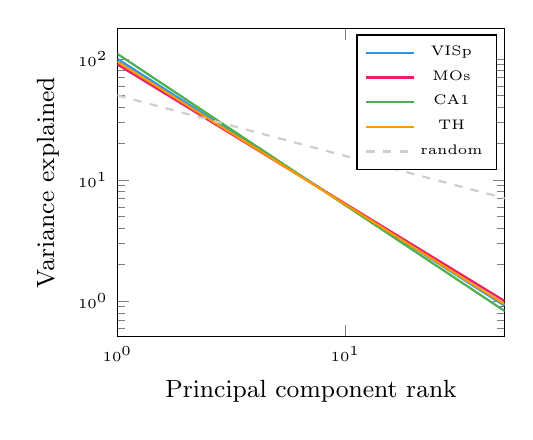
\begin{tikzpicture}
\begin{axis}[
  width=6.5cm, height=5.5cm,
  xlabel={Principal component rank},
  ylabel={Variance explained},
  xlabel style={font=\small},
  ylabel style={font=\small},
  tick label style={font=\tiny},
  xmode=log, ymode=log,
  xmin=1, xmax=50,
  legend style={font=\tiny, at={(0.98,0.98)}, anchor=north east},
]
  \addplot[evidence, thick, domain=1:50, samples=30] {100*x^(-1.2)};
  \addplot[choice, thick, domain=1:50, samples=30] {90*x^(-1.15)};
  \addplot[geometry, thick, domain=1:50, samples=30] {110*x^(-1.25)};
  \addplot[causal, thick, domain=1:50, samples=30] {95*x^(-1.18)};
  \addplot[neutral!50, thick, dashed, domain=1:50, samples=30] {50*x^(-0.5)};
  \legend{VISp, MOs, CA1, TH, random}
\end{axis}
\end{tikzpicture}
\end{column}
\begin{column}{0.48\textwidth}
\textbf{Eigenvalue shape:} $r = 0.936$ across regions \\
{\small Power-law decay is near-identical everywhere}

\vspace{0.8em}
\textbf{Trial-specific content:} $r = 0.089$ \\
{\small Cross-animal similarity of PC projections is low (comparable to permuted-trial null)}

\vspace{1em}
The scaffolding is shared; what gets built on it is region-specific.

\vspace{0.5em}
{\small Subheading: eigenvalue \emph{shape} is universal, but the \emph{modes} are idiosyncratic.}
\end{column}
\end{columns}
\end{frame}

%% ============================================================
%% SLIDE 7: jPCA ROTATION
%% ============================================================

\begin{frame}{Every region rotates (but at different speeds)}
\begin{columns}[T]
\begin{column}{0.5\textwidth}
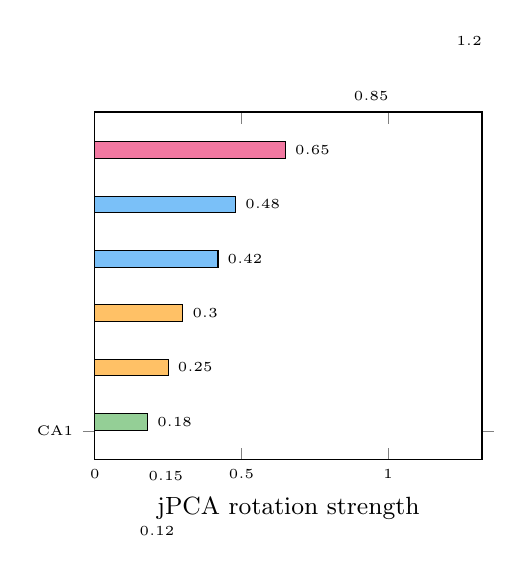
\begin{tikzpicture}
\begin{axis}[
  width=6.5cm, height=6cm,
  xbar,
  bar width=6pt,
  xlabel={jPCA rotation strength},
  xlabel style={font=\small},
  tick label style={font=\tiny},
  symbolic y coords={CA1,DG,SUB,LGd,TH,VISp,VISa,RSP,ACA,MOs},
  ytick=data,
  xmin=0,
  nodes near coords,
  nodes near coords style={font=\tiny},
]
  % Hippocampal (green)
  \addplot[fill=geometry!60] coordinates {(0.12,CA1)};
  \addplot[fill=geometry!60] coordinates {(0.15,DG)};
  \addplot[fill=geometry!60] coordinates {(0.18,SUB)};
  % Thalamic (orange)
  \addplot[fill=causal!60] coordinates {(0.25,LGd)};
  \addplot[fill=causal!60] coordinates {(0.30,TH)};
  % Sensory (blue)
  \addplot[fill=evidence!60] coordinates {(0.42,VISp)};
  \addplot[fill=evidence!60] coordinates {(0.48,VISa)};
  % Frontal (pink)
  \addplot[fill=choice!60] coordinates {(0.65,RSP)};
  \addplot[fill=choice!60] coordinates {(0.85,ACA)};
  \addplot[fill=choice!60] coordinates {(1.20,MOs)};
\end{axis}
\end{tikzpicture}
\end{column}
\begin{column}{0.48\textwidth}
\textbf{72/73 regions} above shuffle null

\vspace{0.5em}
\textbf{10$\times$ variation} in rotation strength

\vspace{0.8em}
\begin{tabular}{ll}
\textcolor{choice}{Frontal/motor} & strongest \\
\textcolor{evidence}{Sensory} & moderate \\
\textcolor{causal}{Thalamic} & moderate \\
\textcolor{geometry}{Hippocampal} & weakest \\
\end{tabular}

\vspace{1em}
{\small Rotational dynamics are ubiquitous but not uniform. The hierarchy is interpretable: motor planning regions rotate fast; memory regions rotate slowly.}

\vspace{0.5em}
{\small \textcolor{neutral}{jPCA, Churchland et al.\ 2012}}
\end{column}
\end{columns}
\end{frame}

%% ============================================================
%% SLIDE 8: ANATOMY RECOVERY (reframed as sanity check)
%% ============================================================

\begin{frame}{Representational similarity matches macro-anatomy}
\begin{columns}[T]
\begin{column}{0.5\textwidth}
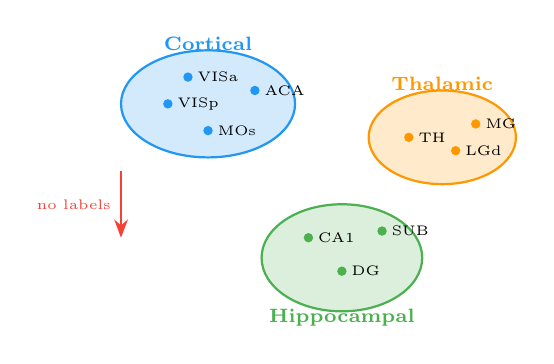
\begin{tikzpicture}[scale=0.85]
  \fill[evidence!20] (-1.5,2) ellipse (1.3 and 0.8);
  \draw[evidence,thick] (-1.5,2) ellipse (1.3 and 0.8);
  \node[evidence,font=\scriptsize\bfseries] at (-1.5,2.9) {Cortical};
  \foreach \name/\x/\y in {VISp/-2.1/2, MOs/-1.5/1.6, ACA/-0.8/2.2, VISa/-1.8/2.4} {
    \fill[evidence] (\x,\y) circle (2pt);
    \node[font=\tiny,right] at (\x,\y) {\name};
  }
  \fill[causal!20] (2,1.5) ellipse (1.1 and 0.7);
  \draw[causal,thick] (2,1.5) ellipse (1.1 and 0.7);
  \node[causal,font=\scriptsize\bfseries] at (2,2.3) {Thalamic};
  \foreach \name/\x/\y in {TH/1.5/1.5, LGd/2.2/1.3, MG/2.5/1.7} {
    \fill[causal] (\x,\y) circle (2pt);
    \node[font=\tiny,right] at (\x,\y) {\name};
  }
  \fill[geometry!20] (0.5,-0.3) ellipse (1.2 and 0.8);
  \draw[geometry,thick] (0.5,-0.3) ellipse (1.2 and 0.8);
  \node[geometry,font=\scriptsize\bfseries] at (0.5,-1.2) {Hippocampal};
  \foreach \name/\x/\y in {CA1/0/0, DG/0.5/-0.5, SUB/1.1/0.1} {
    \fill[geometry] (\x,\y) circle (2pt);
    \node[font=\tiny,right] at (\x,\y) {\name};
  }
  \draw[fail,thick,{Stealth}-] (-2.8,0) -- (-2.8,1) node[midway,left,font=\tiny,fail] {no labels};
\end{tikzpicture}
\end{column}
\begin{column}{0.48\textwidth}
\textbf{Input:} CKA similarity matrix (no anatomy) \\
\textbf{Output:} $k=3$ clusters \\
\textbf{Result:} matches cortical / thalamic / hippocampal

\vspace{0.8em}
Regions with distinct firing statistics and temporal dynamics cluster appropriately. This is \textbf{expected}---but useful as a sanity check that our metric captures biological structure, not noise.

\vspace{0.5em}
{\small Replicates at session level and cross-animal.}
\end{column}
\end{columns}
\end{frame}

%% ============================================================
%% SECTION: CAUSAL INTERVENTIONS
%% ============================================================
\section{Causal interventions}

%% ============================================================
%% SLIDE 9: IIA EXPLANATION
%% ============================================================

\begin{frame}{Interchange Intervention Analysis (IIA)}
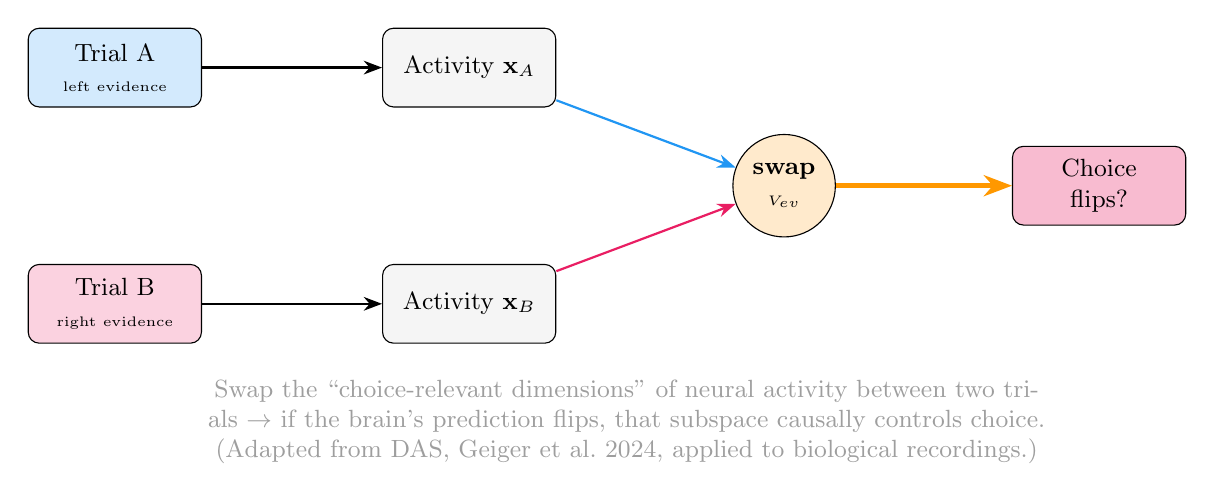
\begin{tikzpicture}[
  box/.style={draw,rounded corners,minimum width=2.2cm,minimum height=1cm,font=\small},
  every node/.style={font=\small},
]
  \node[box,fill=evidence!20,align=center] (trialA) at (0,2) {Trial A \\ {\tiny left evidence}};
  \node[box,fill=choice!20,align=center] (trialB) at (0,-1) {Trial B \\ {\tiny right evidence}};
  \node[box,fill=neutral!10] (actA) at (4.5,2) {Activity $\mathbf{x}_A$};
  \node[box,fill=neutral!10] (actB) at (4.5,-1) {Activity $\mathbf{x}_B$};
  \node[draw,circle,fill=causal!20,minimum size=1.2cm,font=\small\bfseries,align=center] (swap) at (8.5,0.5) {swap \\ {\tiny $V_{ev}$}};
  \node[box,fill=choice!30,align=center] (result) at (12.5,0.5) {Choice \\ flips?};

  \draw[-{Stealth},thick] (trialA) -- (actA);
  \draw[-{Stealth},thick] (trialB) -- (actB);
  \draw[-{Stealth},thick,evidence] (actA) -- (swap);
  \draw[-{Stealth},thick,choice] (actB) -- (swap);
  \draw[-{Stealth},ultra thick,causal] (swap) -- (result);

  \node[font=\small,neutral,text width=12cm,align=center] at (6.5,-2.5) {
    Swap the ``choice-relevant dimensions'' of neural activity between two trials $\to$
    if the brain's prediction flips, that subspace causally controls choice.
    {\small (Adapted from DAS, Geiger et al.\ 2024, applied to biological recordings.)}
  };
\end{tikzpicture}
\end{frame}

%% ============================================================
%% SLIDE 10: IIA RESULTS — with explicit baselines
%% ============================================================

\begin{frame}{IIA: swapping evidence flips choices}
\begin{columns}[T]
\begin{column}{0.5\textwidth}
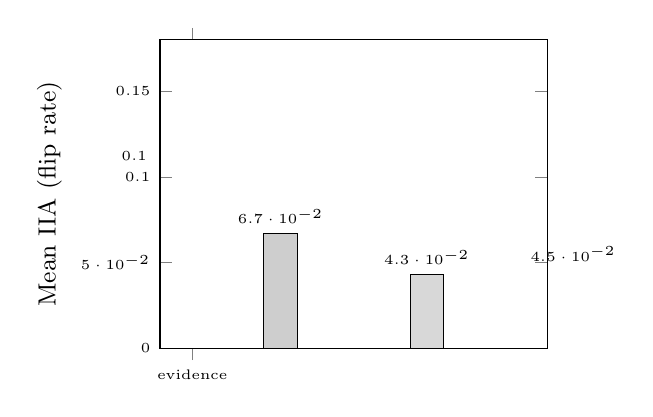
\begin{tikzpicture}
\begin{axis}[
  width=6.5cm, height=5.5cm,
  ybar,
  bar width=12pt,
  ylabel={Mean IIA (flip rate)},
  ylabel style={font=\small},
  tick label style={font=\tiny},
  symbolic x coords={evidence,RT,feedback,random},
  xtick=data,
  ymin=0, ymax=0.18,
  nodes near coords,
  nodes near coords style={font=\tiny},
  every node near coord/.append style={above},
]
  \addplot[fill=evidence] coordinates {(evidence,0.104)};
  \addplot[fill=neutral!50] coordinates {(RT,0.067)};
  \addplot[fill=neutral!40] coordinates {(feedback,0.043)};
  \addplot[fill=neutral!30] coordinates {(random,0.045)};
\end{axis}
\end{tikzpicture}
\end{column}
\begin{column}{0.48\textwidth}
\textbf{Absolute effect:} $\sim$10\% flip rate \\
\textbf{Random baseline:} $\sim$4.5\% flip rate \\
\textbf{Specificity ratio:} 2.3$\times$

\vspace{0.8em}
The effect is modest in absolute terms---but the evidence axis produces more than double the flip rate of random or feedback axes, with $p < 0.001$ (Mann-Whitney).

\vspace{0.8em}
Swapping other axes (RT, feedback, random) produces flip rates near the random baseline. The evidence subspace has a specific causal role.

\vspace{0.5em}
{\small exp49: specificity test}
\end{column}
\end{columns}
\end{frame}

%% ============================================================
%% SLIDE 11: SUFFICIENCY (promoted — strongest single result)
%% ============================================================

\begin{frame}{The evidence subspace is sufficient (and denoises)}
\begin{columns}[T]
\begin{column}{0.5\textwidth}
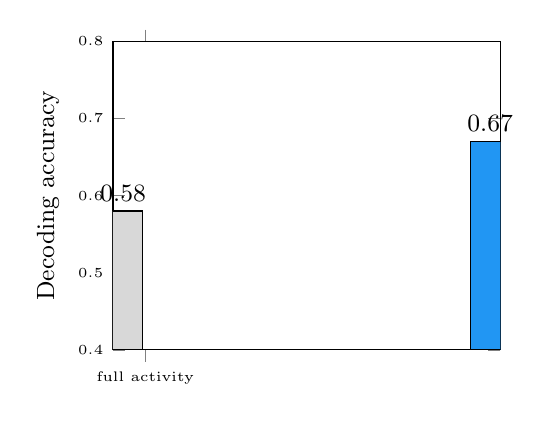
\begin{tikzpicture}
\begin{axis}[
  width=6.5cm, height=5.5cm,
  ybar,
  bar width=14pt,
  ylabel={Decoding accuracy},
  ylabel style={font=\small},
  tick label style={font=\tiny},
  symbolic x coords={full activity, evidence subspace},
  xtick=data,
  ymin=0.4, ymax=0.8,
  nodes near coords,
  nodes near coords style={font=\small},
]
  \addplot[fill=neutral!40] coordinates {(full activity,0.58)};
  \addplot[fill=evidence] coordinates {(evidence subspace,0.67)};
\end{axis}
\end{tikzpicture}
\end{column}
\begin{column}{0.48\textwidth}
\textbf{Recovery fraction = 1.16}

\vspace{0.5em}
The evidence subspace alone decodes choice \emph{better} than full activity---it removes noise dimensions that hurt the classifier.

\vspace{0.8em}
\textbf{20/24 regions pass} ($\geq 0.70$ recovery) \\
{\small 4 failures are all high-dimensional (flat-spectrum) regions where subspace estimation is harder.}

\vspace{0.8em}
Sufficiency + necessity (IIA) together establish the evidence subspace as a causal mediator.

\vspace{0.3em}
{\small exp48}
\end{column}
\end{columns}
\end{frame}

%% ============================================================
%% SLIDE 12: MULTI-METHOD — with explicit naming
%% ============================================================

\begin{frame}{Four intervention methods agree}
\begin{columns}[T]
\begin{column}{0.5\textwidth}
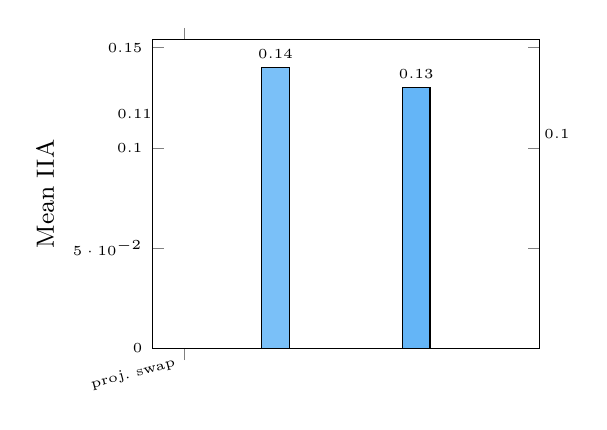
\begin{tikzpicture}
\begin{axis}[
  width=6.5cm, height=5.5cm,
  ybar,
  bar width=10pt,
  ylabel={Mean IIA},
  ylabel style={font=\small},
  tick label style={font=\tiny},
  symbolic x coords={proj.\ swap,noise inj.,mean-shift,zeroing},
  xtick=data,
  xticklabel style={rotate=15,anchor=east,font=\tiny},
  ymin=0,
  nodes near coords,
  nodes near coords style={font=\tiny},
]
  \addplot[fill=evidence!80] coordinates {(proj.\ swap,0.11)};
  \addplot[fill=evidence!60] coordinates {(noise inj.,0.14)};
  \addplot[fill=evidence!70] coordinates {(mean-shift,0.13)};
  \addplot[fill=evidence!50] coordinates {(zeroing,0.10)};
\end{axis}
\end{tikzpicture}
\end{column}
\begin{column}{0.48\textwidth}
\textbf{Methods:}
\begin{enumerate}
  \item \textbf{Projection swap}: replace $V$-projected component
  \item \textbf{Gaussian noise}: add noise along $V$
  \item \textbf{Mean-shift}: shift $V$-projected mean to opposite class
  \item \textbf{Zeroing}: zero out $V$-projected component
\end{enumerate}

\vspace{0.3em}
\textbf{Cross-method rank correlation:} $\bar{\rho} = 0.72$

\vspace{0.3em}
{\small Regions ranking is preserved across methods. The effect is not an artifact of any one intervention type.}

\vspace{0.3em}
{\small exp52: method-invariance test}
\end{column}
\end{columns}
\end{frame}

%% ============================================================
%% SLIDE 13: CONFOUND CONTROL (neuron count moved to limitations)
%% ============================================================

\begin{frame}{Confound control}
\begin{columns}[T]
\begin{column}{0.5\textwidth}
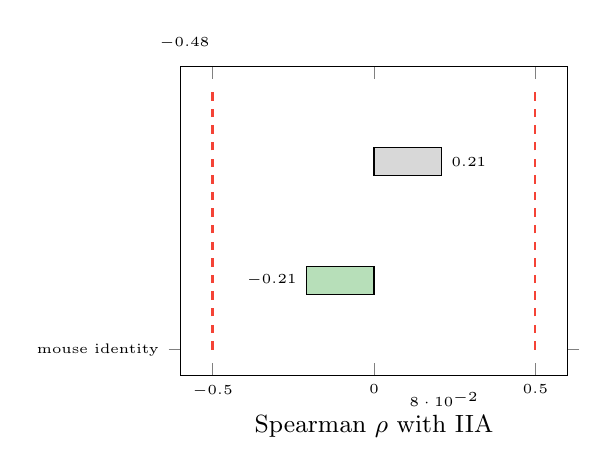
\begin{tikzpicture}
\begin{axis}[
  width=6.5cm, height=5.5cm,
  xbar,
  bar width=10pt,
  xlabel={Spearman $\rho$ with IIA},
  xlabel style={font=\small},
  tick label style={font=\tiny},
  symbolic y coords={mouse identity,trial count,firing rate,neuron count},
  ytick=data,
  xmin=-0.6, xmax=0.6,
  nodes near coords,
  nodes near coords style={font=\tiny},
]
  \addplot[fill=pass!40] coordinates {(0.08,mouse identity)};
  \addplot[fill=pass!40] coordinates {(-0.21,trial count)};
  \addplot[fill=neutral!40] coordinates {(0.21,firing rate)};
  \addplot[fill=partial] coordinates {(-0.48,neuron count)};

  \draw[fail,thick,dashed] (axis cs:0.5,mouse identity) -- (axis cs:0.5,neuron count);
  \draw[fail,thick,dashed] (axis cs:-0.5,mouse identity) -- (axis cs:-0.5,neuron count);
\end{axis}
\end{tikzpicture}
{\small Dashed lines = $|\rho| > 0.5$ threshold}
\end{column}
\begin{column}{0.48\textwidth}
\textbf{No confound exceeds $|\rho| = 0.5$}

\vspace{0.5em}
\begin{itemize}
  \item Firing rate: $\rho = 0.21$ (not significant)
  \item Trial count: $\rho = -0.21$ (not significant)
  \item Mouse identity: $\rho = 0.08$ (effect holds within-mouse)
\end{itemize}

\vspace{0.5em}
\textbf{Caveat:} neuron count shows $\rho = -0.48$---below threshold but a near-miss. Addressed in limitations.

\vspace{0.5em}
{\small exp51}
\end{column}
\end{columns}
\end{frame}

%% ============================================================
%% SLIDE 14: NOVEL PREDICTIONS
%% ============================================================

\begin{frame}{Novel predictions and honest nulls}
\begin{columns}[T]
\begin{column}{0.5\textwidth}
\textbf{Geometric type predicts decoder choice}\\[0.3em]
{\small Regions where CKA is high (linear-type) favor LDA; regions where Procrustes is high (manifold-type) favor kNN. An out-of-sample prediction: geometric type determines which decoder works, without training on decoding data.}

\vspace{0.3em}
\centering $\rho = -0.509$, $p = 0.00016$ {\small ($n = 50$ regions)}

\vspace{0.8em}
\textbf{Causal abstraction geometry}\\[0.3em]
{\small Power-law exponent $\alpha$ correlates with evidence--choice subspace routing.}

\vspace{0.3em}
\centering $\rho = 0.288$, $p = 0.014$ {\small (moderate)}
\end{column}
\begin{column}{0.48\textwidth}
\textbf{Allen Atlas: honest null}\\[0.3em]
{\small Structural connectivity from the Allen Mouse Brain Atlas does not predict functional IIA.}

\vspace{0.3em}
$\rho = 0.031$, $p = 0.65$

\vspace{0.5em}
{\small Anatomical wiring does not predict which regions causally route evidence. The functional geometry we found is not recapitulating known anatomy---it is capturing something different.}

\vspace{0.8em}
{\small \textbf{IBL cross-dataset:} replication in progress (exp46). Results pending.}
\end{column}
\end{columns}
\end{frame}

%% ============================================================
%% SLIDE 15: VALIDITY SCORECARD (standard criterion names)
%% ============================================================

\begin{frame}{Validity scorecard}
{\small
\begin{tabular}{llcl}
\toprule
\textbf{Criterion} & \textbf{Evidence} & \textbf{Status} \\
\midrule
\textbf{Necessity} (IIA) & Flip rate 2.3$\times$ above random & \textcolor{pass}{\textbf{Pass}} \\
\textbf{Sufficiency} & Recovery fraction 1.16 (20/24 regions) & \textcolor{pass}{\textbf{Pass}} \\
\textbf{Specificity} & 4 axes tested, only evidence flips & \textcolor{pass}{\textbf{Pass}} \\
\textbf{Method invariance} & $\bar{\rho} = 0.72$ across 4 methods & \textcolor{pass}{\textbf{Pass}} \\
\textbf{Confound control} & No $|\rho| > 0.5$; neuron count $= -0.48$ & \textcolor{partial}{\textbf{Partial}} \\
\textbf{Double dissociation} & Evidence $\perp$ RT: 18\% dissoc.\ rate & \textcolor{partial}{\textbf{Partial}} \\
\textbf{Cross-dataset} & IBL replication in progress & \textcolor{fail}{\textbf{Not yet}} \\
\midrule
\multicolumn{3}{l}{\textit{Novel predictions}} \\
Geometric type $\to$ decoder & $\rho = -0.51$, $p = 0.0002$ & \textcolor{pass}{\textbf{Pass}} \\
Power-law $\alpha$ $\to$ routing & $\rho = 0.29$, $p = 0.014$ & \textcolor{partial}{\textbf{Moderate}} \\
Allen structural $\to$ functional & $\rho = 0.03$, $p = 0.65$ & \textcolor{fail}{\textbf{Null}} \\
\bottomrule
\end{tabular}
}

\vspace{0.6em}
{\small Criteria adapted from Craver (2007), Shallice (1988), Mayo (2018). We report failures alongside successes.}
\end{frame}

%% ============================================================
%% SECTION: WHAT THIS MEANS
%% ============================================================
\section{What this means}

%% ============================================================
%% SLIDE 16: SUMMARY (claim-precise)
%% ============================================================

\begin{frame}{Summary}
\textbf{What we found:}
\begin{itemize}
  \item CKA and Procrustes systematically disagree ($\rho = -0.85$); effective dimensionality explains why
  \item Rotational dynamics are widespread (72/73 regions) but not uniform (10$\times$ variation)
  \item The evidence subspace causally mediates choice (IIA, 4 methods, sufficiency)
  \item Representational geometry tracks anatomy at the macroscale
\end{itemize}

\vspace{0.8em}
\textbf{What this means:}

\vspace{0.3em}
Neural geometry is \textbf{not metric-neutral}. The tool you choose determines what you find---and dimensionality tells you which tool to use. The causal structure we identify is modest in effect size ($\sim$10\% flip rate) but robust across methods and specific to the evidence axis.
\end{frame}

%% ============================================================
%% SLIDE 17: LIMITATIONS (cleaned up)
%% ============================================================

\begin{frame}{Limitations and next steps}
\begin{columns}[T]
\begin{column}{0.5\textwidth}
\textbf{Honest limitations:}
\begin{itemize}
  \item One dataset (Steinmetz 2019)
  \item Binary task only---unclear if this generalizes
  \item IIA effect sizes are modest ($\sim$10\% flip rate, $\sim$4.5\% baseline)
  \item Double dissociation is partial (18\% rate)
  \item Neuron count $\rho = -0.48$ is a near-miss confound
  \item Exploratory analysis; hypotheses for IBL replication now specified
\end{itemize}
\end{column}
\begin{column}{0.48\textwidth}
\textbf{Next:}
\begin{itemize}
  \item IBL cross-dataset replication (in progress)
  \item Zatka-Haas optogenetic validation \\
    {\small (silencing data downloaded)}
  \item Multi-task generalization
  \item Dimensionality correction for neuron count confound
\end{itemize}
\end{column}
\end{columns}

\vspace{0.8em}
Exploratory work. Code and results are public. Feedback welcome.
\end{frame}

%% ============================================================
%% SLIDE 18: INTELLECTUAL GROUNDING
%% ============================================================

\begin{frame}{Intellectual grounding}
This work draws on ideas from three research traditions:

\vspace{0.5em}
\begin{itemize}
  \item \textbf{Causal representation learning} (Siddharth Mishra-Sharma) --- identifiability conditions for when geometric structure in latent spaces reflects true causal variables
  \item \textbf{Relational causal models} (Jensen \& Neville) --- extending causal inference beyond i.i.d.\ data to relational and multi-level systems, which is what brain region interactions are
  \item \textbf{Dynamical systems in neuroscience} (Hava Siegelmann) --- neural computation as geometry of dynamical trajectories; connections between topology and computational capacity
\end{itemize}

\vspace{0.5em}
Validity framework grounded in philosophy of science (Mayo 2018, Craver 2007, Shallice 1988) and causal inference (Pearl \& Bareinboim 2011, Woodward 2003).
\end{frame}

%% ============================================================
%% SLIDE 19: CLOSING
%% ============================================================

\begin{frame}[standout]
  Code \& results: {\small [ZENODO DOI / GITHUB URL]}

  \vspace{1em}
  Neural geometry is not metric-neutral.\\
  The tool determines the finding---dimensionality tells you which tool to use.
\end{frame}

\end{document}
